\documentclass[1p]{elsarticle_modified}
%\bibliographystyle{elsarticle-num}

%\usepackage[colorlinks]{hyperref}
%\usepackage{abbrmath_seonhwa} %\Abb, \Ascr, \Acal ,\Abf, \Afrak
\usepackage{amsfonts}
\usepackage{amssymb}
\usepackage{amsmath}
\usepackage{amsthm}
\usepackage{scalefnt}
\usepackage{amsbsy}
\usepackage{kotex}
\usepackage{caption}
\usepackage{subfig}
\usepackage{color}
\usepackage{graphicx}
\usepackage{xcolor} %% white, black, red, green, blue, cyan, magenta, yellow
\usepackage{float}
\usepackage{setspace}
\usepackage{hyperref}

\usepackage{tikz}
\usetikzlibrary{arrows}

\usepackage{multirow}
\usepackage{array} % fixed length table
\usepackage{hhline}

%%%%%%%%%%%%%%%%%%%%%
\makeatletter
\renewcommand*\env@matrix[1][\arraystretch]{%
	\edef\arraystretch{#1}%
	\hskip -\arraycolsep
	\let\@ifnextchar\new@ifnextchar
	\array{*\c@MaxMatrixCols c}}
\makeatother %https://tex.stackexchange.com/questions/14071/how-can-i-increase-the-line-spacing-in-a-matrix
%%%%%%%%%%%%%%%

\usepackage[normalem]{ulem}

\newcommand{\msout}[1]{\ifmmode\text{\sout{\ensuremath{#1}}}\else\sout{#1}\fi}
%SOURCE: \msout is \stkout macro in https://tex.stackexchange.com/questions/20609/strikeout-in-math-mode

\newcommand{\cancel}[1]{
	\ifmmode
	{\color{red}\msout{#1}}
	\else
	{\color{red}\sout{#1}}
	\fi
}

\newcommand{\add}[1]{
	{\color{blue}\uwave{#1}}
}

\newcommand{\replace}[2]{
	\ifmmode
	{\color{red}\msout{#1}}{\color{blue}\uwave{#2}}
	\else
	{\color{red}\sout{#1}}{\color{blue}\uwave{#2}}
	\fi
}

\newcommand{\Sol}{\mathcal{S}} %segment
\newcommand{\D}{D} %diagram
\newcommand{\A}{\mathcal{A}} %arc


%%%%%%%%%%%%%%%%%%%%%%%%%%%%%5 test

\def\sl{\operatorname{\textup{SL}}(2,\Cbb)}
\def\psl{\operatorname{\textup{PSL}}(2,\Cbb)}
\def\quan{\mkern 1mu \triangleright \mkern 1mu}

\theoremstyle{definition}
\newtheorem{thm}{Theorem}[section]
\newtheorem{prop}[thm]{Proposition}
\newtheorem{lem}[thm]{Lemma}
\newtheorem{ques}[thm]{Question}
\newtheorem{cor}[thm]{Corollary}
\newtheorem{defn}[thm]{Definition}
\newtheorem{exam}[thm]{Example}
\newtheorem{rmk}[thm]{Remark}
\newtheorem{alg}[thm]{Algorithm}

\newcommand{\I}{\sqrt{-1}}
\begin{document}

%\begin{frontmatter}
%
%\title{Boundary parabolic representations of knots up to 8 crossings}
%
%%% Group authors per affiliation:
%\author{Yunhi Cho} 
%\address{Department of Mathematics, University of Seoul, Seoul, Korea}
%\ead{yhcho@uos.ac.kr}
%
%
%\author{Seonhwa Kim} %\fnref{s_kim}}
%\address{Center for Geometry and Physics, Institute for Basic Science, Pohang, 37673, Korea}
%\ead{ryeona17@ibs.re.kr}
%
%\author{Hyuk Kim}
%\address{Department of Mathematical Sciences, Seoul National University, Seoul 08826, Korea}
%\ead{hyukkim@snu.ac.kr}
%
%\author{Seokbeom Yoon}
%\address{Department of Mathematical Sciences, Seoul National University, Seoul, 08826,  Korea}
%\ead{sbyoon15@snu.ac.kr}
%
%\begin{abstract}
%We find all boundary parabolic representation of knots up to 8 crossings.
%
%\end{abstract}
%\begin{keyword}
%    \MSC[2010] 57M25 
%\end{keyword}
%
%\end{frontmatter}

%\linenumbers
%\tableofcontents
%
\newcommand\colored[1]{\textcolor{white}{\rule[-0.35ex]{0.8em}{1.4ex}}\kern-0.8em\color{red} #1}%
%\newcommand\colored[1]{\textcolor{white}{ #1}\kern-2.17ex	\textcolor{white}{ #1}\kern-1.81ex	\textcolor{white}{ #1}\kern-2.15ex\color{red}#1	}

{\Large $\underline{12a_{1163}~(K12a_{1163})}$}

\setlength{\tabcolsep}{10pt}
\renewcommand{\arraystretch}{1.6}
\vspace{1cm}\begin{tabular}{m{100pt}>{\centering\arraybackslash}m{274pt}}
\multirow{5}{120pt}{
	\centering
	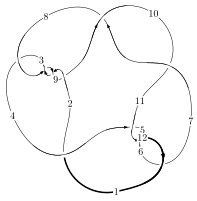
\includegraphics[width=112pt]{../../../GIT/diagram.site/Diagrams/png/1964_12a_1163.png}\\
\ \ \ A knot diagram\footnotemark}&
\allowdisplaybreaks
\textbf{Linearized knot diagam} \\
\cline{2-2}
 &
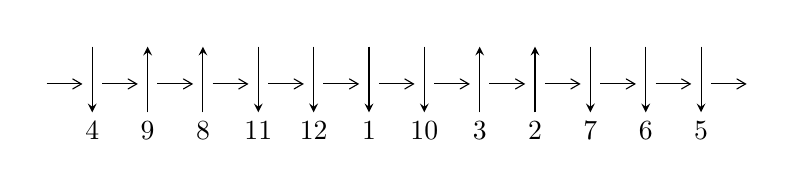
\begin{tikzpicture}[x=20pt, y=17pt]
	% nodes
	\node (C0) at (0, 0) {};
	\node (C1) at (1, 0) {};
	\node (C1U) at (1, +1) {};
	\node (C1D) at (1, -1) {4};

	\node (C2) at (2, 0) {};
	\node (C2U) at (2, +1) {};
	\node (C2D) at (2, -1) {9};

	\node (C3) at (3, 0) {};
	\node (C3U) at (3, +1) {};
	\node (C3D) at (3, -1) {8};

	\node (C4) at (4, 0) {};
	\node (C4U) at (4, +1) {};
	\node (C4D) at (4, -1) {11};

	\node (C5) at (5, 0) {};
	\node (C5U) at (5, +1) {};
	\node (C5D) at (5, -1) {12};

	\node (C6) at (6, 0) {};
	\node (C6U) at (6, +1) {};
	\node (C6D) at (6, -1) {1};

	\node (C7) at (7, 0) {};
	\node (C7U) at (7, +1) {};
	\node (C7D) at (7, -1) {10};

	\node (C8) at (8, 0) {};
	\node (C8U) at (8, +1) {};
	\node (C8D) at (8, -1) {3};

	\node (C9) at (9, 0) {};
	\node (C9U) at (9, +1) {};
	\node (C9D) at (9, -1) {2};

	\node (C10) at (10, 0) {};
	\node (C10U) at (10, +1) {};
	\node (C10D) at (10, -1) {7};

	\node (C11) at (11, 0) {};
	\node (C11U) at (11, +1) {};
	\node (C11D) at (11, -1) {6};

	\node (C12) at (12, 0) {};
	\node (C12U) at (12, +1) {};
	\node (C12D) at (12, -1) {5};
	\node (C13) at (13, 0) {};

	% arrows
	\draw[->,>={angle 60}]
	(C0) edge (C1) (C1) edge (C2) (C2) edge (C3) (C3) edge (C4) (C4) edge (C5) (C5) edge (C6) (C6) edge (C7) (C7) edge (C8) (C8) edge (C9) (C9) edge (C10) (C10) edge (C11) (C11) edge (C12) (C12) edge (C13) ;	\draw[->,>=stealth]
	(C1U) edge (C1D) (C2D) edge (C2U) (C3D) edge (C3U) (C4U) edge (C4D) (C5U) edge (C5D) (C6U) edge (C6D) (C7U) edge (C7D) (C8D) edge (C8U) (C9D) edge (C9U) (C10U) edge (C10D) (C11U) edge (C11D) (C12U) edge (C12D) ;
	\end{tikzpicture} \\
\hhline{~~} \\& 
\textbf{Solving Sequence} \\ \cline{2-2} 
 &
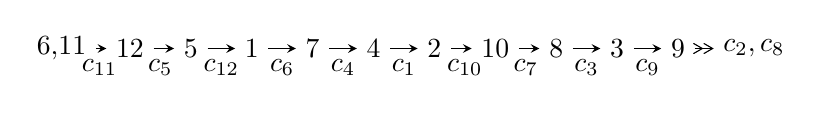
\begin{tikzpicture}[x=22pt, y=7pt]
	% node
	\node (A0) at (-1/8, 0) {6,11};
	\node (A1) at (1, 0) {12};
	\node (A2) at (2, 0) {5};
	\node (A3) at (3, 0) {1};
	\node (A4) at (4, 0) {7};
	\node (A5) at (5, 0) {4};
	\node (A6) at (6, 0) {2};
	\node (A7) at (7, 0) {10};
	\node (A8) at (8, 0) {8};
	\node (A9) at (9, 0) {3};
	\node (A10) at (10, 0) {9};
	\node (C1) at (1/2, -1) {$c_{11}$};
	\node (C2) at (3/2, -1) {$c_{5}$};
	\node (C3) at (5/2, -1) {$c_{12}$};
	\node (C4) at (7/2, -1) {$c_{6}$};
	\node (C5) at (9/2, -1) {$c_{4}$};
	\node (C6) at (11/2, -1) {$c_{1}$};
	\node (C7) at (13/2, -1) {$c_{10}$};
	\node (C8) at (15/2, -1) {$c_{7}$};
	\node (C9) at (17/2, -1) {$c_{3}$};
	\node (C10) at (19/2, -1) {$c_{9}$};
	\node (A11) at (45/4, 0) {$c_{2},c_{8}$};

	% edge
	\draw[->,>=stealth]	
	(A0) edge (A1) (A1) edge (A2) (A2) edge (A3) (A3) edge (A4) (A4) edge (A5) (A5) edge (A6) (A6) edge (A7) (A7) edge (A8) (A8) edge (A9) (A9) edge (A10) ;
	\draw[->>,>={angle 60}]	
	(A10) edge (A11);
\end{tikzpicture} \\ 

\end{tabular} \\

\footnotetext{
The image of knot diagram is generated by the software ``\textbf{Draw programme}" developed by Andrew Bartholomew(\url{http://www.layer8.co.uk/maths/draw/index.htm\#Running-draw}), where we modified some parts for our purpose(\url{https://github.com/CATsTAILs/LinksPainter}).
}\phantom \\ \newline 
\centering \textbf{Ideals for irreducible components\footnotemark of $X_{\text{par}}$} 
 
\begin{align*}
I^u_{1}&=\langle 
u^{51}- u^{50}+\cdots+2 u-1\rangle \\
\\
\end{align*}
\raggedright * 1 irreducible components of $\dim_{\mathbb{C}}=0$, with total 51 representations.\\
\footnotetext{All coefficients of polynomials are rational numbers. But the coefficients are sometimes approximated in decimal forms when there is not enough margin.}
\newpage
\renewcommand{\arraystretch}{1}
\centering \section*{I. $I^u_{1}= \langle u^{51}- u^{50}+\cdots+2 u-1 \rangle$}
\flushleft \textbf{(i) Arc colorings}\\
\begin{tabular}{m{7pt} m{180pt} m{7pt} m{180pt} }
\flushright $a_{6}=$&$\begin{pmatrix}0\\u\end{pmatrix}$ \\
\flushright $a_{11}=$&$\begin{pmatrix}1\\0\end{pmatrix}$ \\
\flushright $a_{12}=$&$\begin{pmatrix}1\\u^2\end{pmatrix}$ \\
\flushright $a_{5}=$&$\begin{pmatrix}u\\u^3+u\end{pmatrix}$ \\
\flushright $a_{1}=$&$\begin{pmatrix}u^2+1\\u^4+2 u^2\end{pmatrix}$ \\
\flushright $a_{7}=$&$\begin{pmatrix}- u^5-2 u^3- u\\- u^7-3 u^5-2 u^3+u\end{pmatrix}$ \\
\flushright $a_{4}=$&$\begin{pmatrix}u^3+2 u\\u^3+u\end{pmatrix}$ \\
\flushright $a_{2}=$&$\begin{pmatrix}- u^{10}-5 u^8-8 u^6-3 u^4+3 u^2+1\\- u^{10}-4 u^8-5 u^6+3 u^2\end{pmatrix}$ \\
\flushright $a_{10}=$&$\begin{pmatrix}- u^{12}-5 u^{10}-9 u^8-6 u^6+u^2+1\\- u^{14}-6 u^{12}-13 u^{10}-10 u^8+2 u^6+4 u^4- u^2\end{pmatrix}$ \\
\flushright $a_{8}=$&$\begin{pmatrix}- u^{19}-8 u^{17}-26 u^{15}-42 u^{13}-31 u^{11}-2 u^9+10 u^7+4 u^5- u^3-2 u\\- u^{21}-9 u^{19}+\cdots- u^3+u\end{pmatrix}$ \\
\flushright $a_{3}=$&$\begin{pmatrix}u^{43}+18 u^{41}+\cdots-7 u^3+2 u\\u^{45}+19 u^{43}+\cdots+5 u^3+u\end{pmatrix}$ \\
\flushright $a_{9}=$&$\begin{pmatrix}u^{34}+15 u^{32}+\cdots+5 u^2+1\\u^{34}+14 u^{32}+\cdots+16 u^4- u^2\end{pmatrix}$\\&\end{tabular}
\flushleft \textbf{(ii) Obstruction class $= -1$}\\~\\
\flushleft \textbf{(iii) Cusp Shapes $= -4 u^{50}+4 u^{49}+\cdots+20 u-6$}\\~\\
\newpage\renewcommand{\arraystretch}{1}
\flushleft \textbf{(iv) u-Polynomials at the component}\newline \\
\begin{tabular}{m{50pt}|m{274pt}}
Crossings & \hspace{64pt}u-Polynomials at each crossing \\
\hline $$\begin{aligned}c_{1},c_{7},c_{10}\end{aligned}$$&$\begin{aligned}
&u^{51}-7 u^{50}+\cdots+112 u-17
\end{aligned}$\\
\hline $$\begin{aligned}c_{2},c_{3},c_{8}\\c_{9}\end{aligned}$$&$\begin{aligned}
&u^{51}+u^{50}+\cdots+3 u^2+1
\end{aligned}$\\
\hline $$\begin{aligned}c_{4},c_{6}\end{aligned}$$&$\begin{aligned}
&u^{51}- u^{50}+\cdots+3 u^2+1
\end{aligned}$\\
\hline $$\begin{aligned}c_{5},c_{11},c_{12}\end{aligned}$$&$\begin{aligned}
&u^{51}+u^{50}+\cdots+2 u+1
\end{aligned}$\\
\hline
\end{tabular}\\~\\
\newpage\renewcommand{\arraystretch}{1}
\flushleft \textbf{(v) Riley Polynomials at the component}\newline \\
\begin{tabular}{m{50pt}|m{274pt}}
Crossings & \hspace{64pt}Riley Polynomials at each crossing \\
\hline $$\begin{aligned}c_{1},c_{7},c_{10}\end{aligned}$$&$\begin{aligned}
&y^{51}+47 y^{50}+\cdots+202 y-289
\end{aligned}$\\
\hline $$\begin{aligned}c_{2},c_{3},c_{8}\\c_{9}\end{aligned}$$&$\begin{aligned}
&y^{51}+55 y^{50}+\cdots-6 y-1
\end{aligned}$\\
\hline $$\begin{aligned}c_{4},c_{6}\end{aligned}$$&$\begin{aligned}
&y^{51}-25 y^{50}+\cdots-6 y-1
\end{aligned}$\\
\hline $$\begin{aligned}c_{5},c_{11},c_{12}\end{aligned}$$&$\begin{aligned}
&y^{51}+43 y^{50}+\cdots-6 y-1
\end{aligned}$\\
\hline
\end{tabular}\\~\\
\newpage\flushleft \textbf{(vi) Complex Volumes and Cusp Shapes}
$$\begin{array}{c|c|c}  
\text{Solutions to }I^u_{1}& \I (\text{vol} + \sqrt{-1}CS) & \text{Cusp shape}\\
 \hline 
\begin{aligned}
u &= -0.249709 + 0.948226 I\end{aligned}
 & \phantom{-}4.63631 - 2.12088 I & -1.01844 + 2.80811 I \\ \hline\begin{aligned}
u &= -0.249709 - 0.948226 I\end{aligned}
 & \phantom{-}4.63631 + 2.12088 I & -1.01844 - 2.80811 I \\ \hline\begin{aligned}
u &= \phantom{-}0.295729 + 0.994644 I\end{aligned}
 & -2.13539 + 4.89833 I & -5.01649 - 2.19451 I \\ \hline\begin{aligned}
u &= \phantom{-}0.295729 - 0.994644 I\end{aligned}
 & -2.13539 - 4.89833 I & -5.01649 + 2.19451 I \\ \hline\begin{aligned}
u &= \phantom{-}0.230603 + 0.853532 I\end{aligned}
 & \phantom{-}4.74743 - 1.96048 I & -0.34668 + 4.23406 I \\ \hline\begin{aligned}
u &= \phantom{-}0.230603 - 0.853532 I\end{aligned}
 & \phantom{-}4.74743 + 1.96048 I & -0.34668 - 4.23406 I \\ \hline\begin{aligned}
u &= -0.273056 + 0.774265 I\end{aligned}
 & -1.78828 + 4.72311 I & -4.06394 - 4.26663 I \\ \hline\begin{aligned}
u &= -0.273056 - 0.774265 I\end{aligned}
 & -1.78828 - 4.72311 I & -4.06394 + 4.26663 I \\ \hline\begin{aligned}
u &= \phantom{-}0.777766 + 0.178377 I\end{aligned}
 & -4.65007 - 8.93459 I & -8.10474 + 6.18574 I \\ \hline\begin{aligned}
u &= \phantom{-}0.777766 - 0.178377 I\end{aligned}
 & -4.65007 + 8.93459 I & -8.10474 - 6.18574 I \\ \hline\begin{aligned}
u &= -0.761639 + 0.184556 I\end{aligned}
 & \phantom{-}2.23741 + 6.02041 I & -4.49356 - 6.91985 I \\ \hline\begin{aligned}
u &= -0.761639 - 0.184556 I\end{aligned}
 & \phantom{-}2.23741 - 6.02041 I & -4.49356 + 6.91985 I \\ \hline\begin{aligned}
u &= \phantom{-}0.775098 + 0.060463 I\end{aligned}
 & -11.25330 - 3.44491 I & -12.79521 + 3.55577 I \\ \hline\begin{aligned}
u &= \phantom{-}0.775098 - 0.060463 I\end{aligned}
 & -11.25330 + 3.44491 I & -12.79521 - 3.55577 I \\ \hline\begin{aligned}
u &= \phantom{-}0.742257 + 0.192170 I\end{aligned}
 & \phantom{-}2.53020 - 1.80186 I & -3.57173 + 0.69342 I \\ \hline\begin{aligned}
u &= \phantom{-}0.742257 - 0.192170 I\end{aligned}
 & \phantom{-}2.53020 + 1.80186 I & -3.57173 - 0.69342 I \\ \hline\begin{aligned}
u &= \phantom{-}0.318281 + 1.201370 I\end{aligned}
 & -7.76752 - 0.51963 I & \phantom{-0.000000 } 0 \\ \hline\begin{aligned}
u &= \phantom{-}0.318281 - 1.201370 I\end{aligned}
 & -7.76752 + 0.51963 I & \phantom{-0.000000 } 0 \\ \hline\begin{aligned}
u &= -0.275754 + 1.221110 I\end{aligned}
 & -0.186542 + 1.326290 I & \phantom{-0.000000 } 0 \\ \hline\begin{aligned}
u &= -0.275754 - 1.221110 I\end{aligned}
 & -0.186542 - 1.326290 I & \phantom{-0.000000 } 0 \\ \hline\begin{aligned}
u &= -0.716310 + 0.207468 I\end{aligned}
 & -3.73927 - 1.03700 I & -7.10850 - 0.87605 I \\ \hline\begin{aligned}
u &= -0.716310 - 0.207468 I\end{aligned}
 & -3.73927 + 1.03700 I & -7.10850 + 0.87605 I \\ \hline\begin{aligned}
u &= \phantom{-}0.063850 + 1.258910 I\end{aligned}
 & \phantom{-}4.32614 - 1.52805 I & \phantom{-0.000000 } 0 \\ \hline\begin{aligned}
u &= \phantom{-}0.063850 - 1.258910 I\end{aligned}
 & \phantom{-}4.32614 + 1.52805 I & \phantom{-0.000000 } 0 \\ \hline\begin{aligned}
u &= -0.731823 + 0.057552 I\end{aligned}
 & -3.72646 + 2.32596 I & -11.41052 - 5.70564 I \\ \hline\begin{aligned}
u &= -0.731823 - 0.057552 I\end{aligned}
 & -3.72646 - 2.32596 I & -11.41052 + 5.70564 I \\ \hline\begin{aligned}
u &= \phantom{-}0.267337 + 1.286100 I\end{aligned}
 & \phantom{-}2.27908 - 3.39012 I & \phantom{-0.000000 } 0 \\ \hline\begin{aligned}
u &= \phantom{-}0.267337 - 1.286100 I\end{aligned}
 & \phantom{-}2.27908 + 3.39012 I & \phantom{-0.000000 } 0 \\ \hline\begin{aligned}
u &= -0.145806 + 1.317740 I\end{aligned}
 & -1.58295 + 3.13834 I & \phantom{-0.000000 } 0 \\ \hline\begin{aligned}
u &= -0.145806 - 1.317740 I\end{aligned}
 & -1.58295 - 3.13834 I & \phantom{-0.000000 } 0\\
 \hline 
 \end{array}$$\newpage$$\begin{array}{c|c|c}  
\text{Solutions to }I^u_{1}& \I (\text{vol} + \sqrt{-1}CS) & \text{Cusp shape}\\
 \hline 
\begin{aligned}
u &= \phantom{-}0.671685\phantom{ +0.000000I}\end{aligned}
 & -1.74026\phantom{ +0.000000I} & -4.25130\phantom{ +0.000000I} \\ \hline\begin{aligned}
u &= -0.306268 + 1.301300 I\end{aligned}
 & \phantom{-}0.52039 + 6.08284 I & \phantom{-0.000000 } 0 \\ \hline\begin{aligned}
u &= -0.306268 - 1.301300 I\end{aligned}
 & \phantom{-}0.52039 - 6.08284 I & \phantom{-0.000000 } 0 \\ \hline\begin{aligned}
u &= \phantom{-}0.332711 + 1.301130 I\end{aligned}
 & -7.00145 - 7.44226 I & \phantom{-0.000000 } 0 \\ \hline\begin{aligned}
u &= \phantom{-}0.332711 - 1.301130 I\end{aligned}
 & -7.00145 + 7.44226 I & \phantom{-0.000000 } 0 \\ \hline\begin{aligned}
u &= -0.297050 + 1.372640 I\end{aligned}
 & \phantom{-}1.25075 + 2.64872 I & \phantom{-0.000000 } 0 \\ \hline\begin{aligned}
u &= -0.297050 - 1.372640 I\end{aligned}
 & \phantom{-}1.25075 - 2.64872 I & \phantom{-0.000000 } 0 \\ \hline\begin{aligned}
u &= \phantom{-}0.309777 + 1.371410 I\end{aligned}
 & \phantom{-}7.47174 - 5.62076 I & \phantom{-0.000000 } 0 \\ \hline\begin{aligned}
u &= \phantom{-}0.309777 - 1.371410 I\end{aligned}
 & \phantom{-}7.47174 + 5.62076 I & \phantom{-0.000000 } 0 \\ \hline\begin{aligned}
u &= -0.319107 + 1.370980 I\end{aligned}
 & \phantom{-}7.15390 + 9.93639 I & \phantom{-0.000000 } 0 \\ \hline\begin{aligned}
u &= -0.319107 - 1.370980 I\end{aligned}
 & \phantom{-}7.15390 - 9.93639 I & \phantom{-0.000000 } 0 \\ \hline\begin{aligned}
u &= \phantom{-}0.327378 + 1.370270 I\end{aligned}
 & \phantom{-}0.24340 - 12.93330 I & \phantom{-0.000000 } 0 \\ \hline\begin{aligned}
u &= \phantom{-}0.327378 - 1.370270 I\end{aligned}
 & \phantom{-}0.24340 + 12.93330 I & \phantom{-0.000000 } 0 \\ \hline\begin{aligned}
u &= \phantom{-}0.00618 + 1.42442 I\end{aligned}
 & \phantom{-}11.54180 - 2.18033 I & \phantom{-0.000000 } 0 \\ \hline\begin{aligned}
u &= \phantom{-}0.00618 - 1.42442 I\end{aligned}
 & \phantom{-}11.54180 + 2.18033 I & \phantom{-0.000000 } 0 \\ \hline\begin{aligned}
u &= -0.01946 + 1.42477 I\end{aligned}
 & \phantom{-}4.94539 + 5.22241 I & \phantom{-0.000000 } 0 \\ \hline\begin{aligned}
u &= -0.01946 - 1.42477 I\end{aligned}
 & \phantom{-}4.94539 - 5.22241 I & \phantom{-0.000000 } 0 \\ \hline\begin{aligned}
u &= -0.374516 + 0.344098 I\end{aligned}
 & -6.57378 + 1.34480 I & -7.53020 - 4.73780 I \\ \hline\begin{aligned}
u &= -0.374516 - 0.344098 I\end{aligned}
 & -6.57378 - 1.34480 I & -7.53020 + 4.73780 I \\ \hline\begin{aligned}
u &= \phantom{-}0.187694 + 0.267286 I\end{aligned}
 & -0.141288 - 0.746703 I & -4.42303 + 9.26587 I \\ \hline\begin{aligned}
u &= \phantom{-}0.187694 - 0.267286 I\end{aligned}
 & -0.141288 + 0.746703 I & -4.42303 - 9.26587 I\\
 \hline 
 \end{array}$$\newpage
\newpage\renewcommand{\arraystretch}{1}
\centering \section*{ II. u-Polynomials}
\begin{tabular}{m{50pt}|m{274pt}}
Crossings & \hspace{64pt}u-Polynomials at each crossing \\
\hline $$\begin{aligned}c_{1},c_{7},c_{10}\end{aligned}$$&$\begin{aligned}
&u^{51}-7 u^{50}+\cdots+112 u-17
\end{aligned}$\\
\hline $$\begin{aligned}c_{2},c_{3},c_{8}\\c_{9}\end{aligned}$$&$\begin{aligned}
&u^{51}+u^{50}+\cdots+3 u^2+1
\end{aligned}$\\
\hline $$\begin{aligned}c_{4},c_{6}\end{aligned}$$&$\begin{aligned}
&u^{51}- u^{50}+\cdots+3 u^2+1
\end{aligned}$\\
\hline $$\begin{aligned}c_{5},c_{11},c_{12}\end{aligned}$$&$\begin{aligned}
&u^{51}+u^{50}+\cdots+2 u+1
\end{aligned}$\\
\hline
\end{tabular}\newpage\renewcommand{\arraystretch}{1}
\centering \section*{ III. Riley Polynomials}
\begin{tabular}{m{50pt}|m{274pt}}
Crossings & \hspace{64pt}Riley Polynomials at each crossing \\
\hline $$\begin{aligned}c_{1},c_{7},c_{10}\end{aligned}$$&$\begin{aligned}
&y^{51}+47 y^{50}+\cdots+202 y-289
\end{aligned}$\\
\hline $$\begin{aligned}c_{2},c_{3},c_{8}\\c_{9}\end{aligned}$$&$\begin{aligned}
&y^{51}+55 y^{50}+\cdots-6 y-1
\end{aligned}$\\
\hline $$\begin{aligned}c_{4},c_{6}\end{aligned}$$&$\begin{aligned}
&y^{51}-25 y^{50}+\cdots-6 y-1
\end{aligned}$\\
\hline $$\begin{aligned}c_{5},c_{11},c_{12}\end{aligned}$$&$\begin{aligned}
&y^{51}+43 y^{50}+\cdots-6 y-1
\end{aligned}$\\
\hline
\end{tabular}
\vskip 2pc
\end{document}